\documentclass{article}
\usepackage{graphics} 
\usepackage{hyperref}
\usepackage{fixltx2e}
\usepackage{amssymb}
\usepackage{tikz}
\usepackage{amsmath}

\author{Kevin Zollicoffer}
\title{Data Mining in R\\Assignment 3}
\date{2/03/2014}

% no indents
\setlength\parindent{0pt}

\usepackage{Sweave}
\begin{document}
\maketitle
%\tableofcontents
\Sconcordance{concordance:KevinZollicoffer_Assignment3.tex:KevinZollicoffer_Assignment3.Rnw:%
1 15 1 1 0 33 1 1 2 4 0 1 2 2 1 1 3 5 0 1 2 2 1 1 2 1 0 1 1 12 0 1 2 2 %
1 1 2 1 0 1 1 11 0 1 2 2 1 1 2 1 0 1 1 11 0 1 2 2 1 1 2 4 0 2 2 1 0 1 1 %
11 0 1 2 2 1 1 2 1 0 2 1 4 0 1 2 2 1}


\section*{Q.1}
Supervised tasks are learning tasks where a model is trained to find a target variable given 1 or more predictors. A supervised model is trained with data where the target is known so that it can predict a target with a new set of predictor variables where the target is unknown. 

Unsupervised tasks are used where the data contains only descriptive variables where the data is unclassified. There is no learning phase as there is no information about possible target variables or outcomes. 

\section*{Q.2}
Both clustering and outlier detection attempt to find natural groupings of a set of observations that are similar to each other. In the case of outlier detection, the natural grouping of outliers may be due to their similarity in the distance away from some measure of the center of the observations distribution. 

The notion of similarity in clustering usually requires the definition of a metric over the space defined by the variables that describe the observations. Similarly, outliers can be detected by a measure of their distance away from other observations. 

\section*{Q.3}
Classification accuracy measures the proportion of successful classification to the total size of the observation set. In a classification problem with imbalanced class distributions Classification Accuracy can be skewed by the dominant, most likely class. 

Precision measures the proportion of a models predicted target class to the actual true number of the test sets target class. That is, given an input test sets true number of target classifications, what proportion was the model able to accurately predict.  

\section*{Q.4}
We would need more information to properly measure model quality. However, precision is likely very low with 100\% recall, and therefore model quality low. The reason is that to achieve recall of 100\% the model is likely predicting a high degree of non-fraud cases as fraud diminishing the predictive value of the model. 

\section*{Q.5}
The dominate class can skew results. For example, in the fraud detection case in this lesson, the non-fraud transactions will overwhelm the fraud transactions and the classification accuracy calculation will turn out high as most transactions are indeed not fraud. But this does not nesscarily mean our model is good at predicting fraud. It may just be good at the much easier task of spotting non-fraud - the most likely classification of a transaction. 

\section*{Q.6}
The cross validation method randomly samples it's k subsets of data from the same training set. This is most suitable when the size of the training data set is not suitable to the hold out method due to concerns in achiveing measures that are statistically significant.  

The hold out method divides the availble data into at least a training set, and test set. The training and test data sets do not intersect. The hold out method is more suitable to large data sets where achieving measures that are statistically significant are not a concern. 

\section*{Assignment}
First load the data

\begin{Schunk}
\begin{Sinput}
> load("sales.Rdata")
\end{Sinput}
\end{Schunk}

We need the proportion of products sold to the total products available so lets store off total products. 

\begin{Schunk}
\begin{Sinput}
> # total products
> prods.total <- nlevels(sales$Prod)
\end{Sinput}
\end{Schunk}

Next, we sum total sales by salesperson ID

\begin{Schunk}
\begin{Sinput}
> sales.agg <- aggregate(sales$Quant, list(sales$ID), sum, na.rm=T)
> head(sales.agg)
\end{Sinput}
\begin{Soutput}
  Group.1      x
1      v1  53517
2      v2 273352
3      v3 102083
4      v4  78069
5      v5   3668
6      v6 238957
\end{Soutput}
\end{Schunk}

Now get top 5 salespersons

\begin{Schunk}
\begin{Sinput}
> sales.top5 <- sales.agg[order(sales.agg$x, decreasing=T),][1:5,]
> sales.top5
\end{Sinput}
\begin{Soutput}
     Group.1         x
5420   v5458 546932272
5686   v5733 473926684
3882   v3901 206186227
242     v243 181099126
3911   v3930 113623819
\end{Soutput}
\end{Schunk}

Here we give better column names

\begin{Schunk}
\begin{Sinput}
> names(sales.top5) <- c('ID','Quant')
> sales.top5
\end{Sinput}
\begin{Soutput}
        ID     Quant
5420 v5458 546932272
5686 v5733 473926684
3882 v3901 206186227
242   v243 181099126
3911 v3930 113623819
\end{Soutput}
\end{Schunk}

Cummulative stats for the top 5 salespersons

\begin{Schunk}
\begin{Sinput}
> sales.top5.all <- sales[sales$ID %in% sales.top5$ID,]
\end{Sinput}
\end{Schunk}

\begin{Schunk}
\begin{Sinput}
> sales.top5.div <- aggregate(Prod ~ ID, data=sales.top5.all, FUN=function(x) length(unique(x)))
> sales.top5.div
\end{Sinput}
\begin{Soutput}
     ID Prod
1  v243    6
2 v3901    7
3 v3930    2
4 v5458    2
5 v5733   58
\end{Soutput}
\end{Schunk}

And finally we get the diversity of the product portfolio of the top 5 salesman as a proportion of all products that the salesmen sold over total products available to sale.

\begin{Schunk}
\begin{Sinput}
> par(mfrow=c(1,1))
> sales.top5.div <- aggregate(Prod ~ ID, data=sales.top5.all, FUN=function(x) length(unique(x))/prods.total)
> barplot(as.table(sales.top5.div$Prod), main="Top 5 salesperson product diversity", names.arg=sales.top5.div$ID, xlab="Salesperson ID", ylab="Proportion of total product")
\end{Sinput}
\end{Schunk}
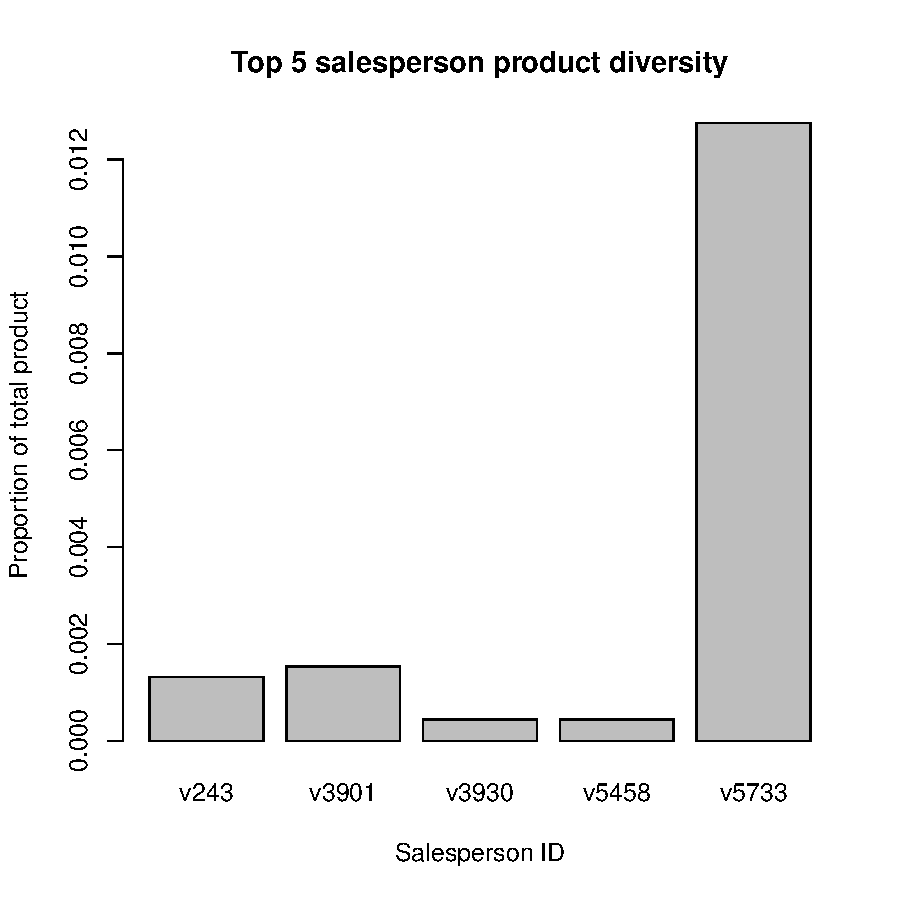
\includegraphics{KevinZollicoffer_Assignment3-008}


\end{document}
